\documentclass[12pt,a4paper]{instrumentacao}

\title{Alguns dos Efeitos Físicos Explorados em Sensores}
\author{Rogiel Sulzbach \and Rodrigo de Castro Silveira \and Yi Chen Wu}
\startdate{28 de março de 2016}
\finishdate{04 de abril de 2016}
\emails{
	\emailaddress{R.J.S.}{rogiel@rogiel.com},
	\emailaddress{R.C.S.}{csilveira.rodrigo@gmail.com} e
	\emailaddress{Y.C.}{yichen.wu@ufrgs.br}
}
\resume{}
\abstract{}
\keywords{}
\institute{Universidade Federal do Rio Grande do Sul, Departamento de Engenharia Elétrica, Curso de Engenharia Elétrica, Instrumentação A, Profs. Dr. Alexandre Balbinot e Dra. Léia Bagesteiro}

\headertext{Efeitos físicos}

\begin{document}
\maketitle

\todo{mudar a letra para times new roman.......}

\chapter{Introdução}
Nesta atividade de laboratório exploramos os efeitos físicos de dois tipos de sensores. Um sensor potenciométrico e outro de efeito Hall linear.

\chapter{Metodologia Experimental}
\section{Sensor potênciométrico}
Para a atividade do sensor potenciométrico, desenvolvemos um pêndulo cujo eixo estava conectado à um potenciômetro. A construção está ilustrada na figura \ref{fig:estrutura-pendulo}:

\begin{figure}[H]
\centering
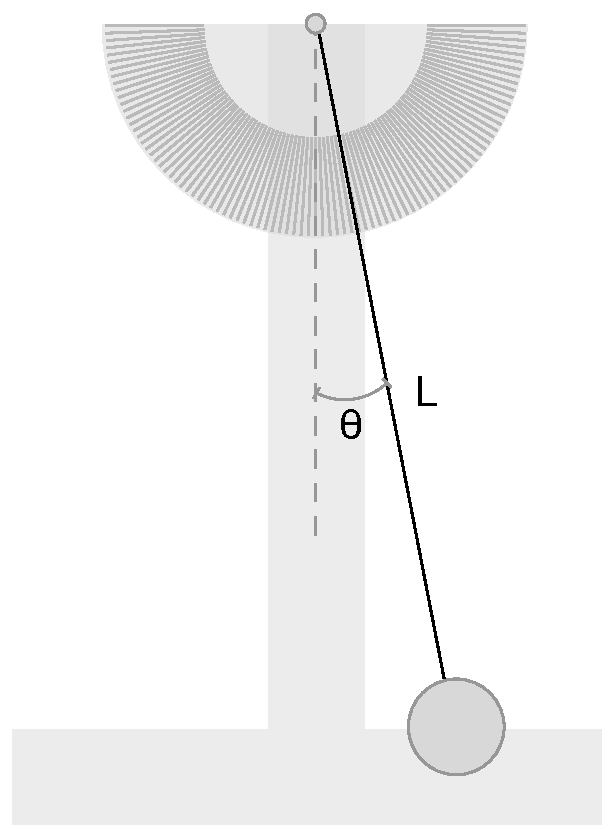
\includegraphics[width=0.4\textwidth]{images/Pendulo.pdf}
\caption{Estrutura do pêndulo}
\label{fig:pendulo}
\end{figure}

onde $\theta$ é o angulo de inclinação do pêndulo em relação a origem (linha tracejada).

\todo{equacionamento do pendulo}

Primeiramente, a fim de obter uma curva de calibração da estrutura, se fez necessário levantar estimativas do valor de resistência \todo{ou tensão} do potenciômetro em função do seu ângulo de oscilação. A fim de conseguir realizar o projeto em tempo hábil \todo{colocar isso mesmo?}, optamos por realizar as medidas em intervalos de 10 em 10 graus de inclinação no intervalo de -80º (oscilação ao lado esquerdo) e 80º (oscilação ao lado direito).

Com estes dados, e assumindo que o potenciômetro seja linear, podemos assumir que os valores intermediários de tensão mensuradas são proporcionais aos seus limites mensurados (valor medido superior e inferior).

\chapter{Resultados e Discussões}

Com o pêndulo alimentado com a tensão elétrica simétrica de -5V e +5V, levantamos as seguintes medidas a fim de obter uma relação de tensão elétrica em função do angulo do pêndulo. A tabela \ref{tab:pendulo-calibracao} contém as medidas obtidas:

\begin{table}[H]
\centering
\caption{Tabela da relação entre temperatura e a resistência elétrica medida}
\begin{tabular}{|l|l|l|}
 \hline
 \textbf{Ângulo ($º$)} & \textbf{Tensão Elétrica ($V$)} & \textbf{Tensão Elétrica ($V$)} \\ \hline

 -60 & -1.886 & -1.886 	\\ \hline
 -55 & -1.702 & -1.702 	\\ \hline
 -50 & -1.564 & -1.564 	\\ \hline
 -45 & -1.426 & -1.426 	\\ \hline
 -40 & -1.196 & -1.196 	\\ \hline
 -35 & -1.127 & -1.127 	\\ \hline
 -30 & -0.92 & -0.92 	\\ \hline
 -25 & -0.736 & -0.736 	\\ \hline
 -20 & -0.621 & -0.621 	\\ \hline
 -15 & -0.46 & -0.46 	\\ \hline
 -10 & -0.345 & -0.345 	\\ \hline
 -5 & -0.184 & -0.184 	\\ \hline
 0 & 0. & 0. 			\\ \hline
 5 & 0.138 & 0.138 		\\ \hline
 10 & 0.322 & 0.322 	\\ \hline
 15 & 0.506 & 0.506 	\\ \hline
 20 & 0.69 & 0.69 		\\ \hline
 25 & 0.828 & 0.828 	\\ \hline
 30 & 0.966 & 0.966 	\\ \hline
 35 & 1.127 & 1.127 	\\ \hline
 40 & 1.265 & 1.265 	\\ \hline
 45 & 1.472 & 1.472 	\\ \hline
 50 & 1.587 & 1.587 	\\ \hline
 55 & 1.84 & 1.84 		\\ \hline
 60 & 1.955 & 1.955 	\\ \hline
 
\end{tabular}
\label{tab:pendulo-calibracao}
\end{table}
\todo{okay, essa tabela ta totalmente errada. temos que refazer o experimento.} % eu fiz uma multiplicação mágica pra ajustar os valores que teríamos medido, mas precisamos mesmo fazer a medida certa dessa coisa, ou o Balbinot não vai aceitar

Observa-se que cada medida foi feita com duas repetições e de forma totalmente aleatória.

Podemos, adicionalmente, plotar estes pontos em um gráfico para melhor observar o formato da curva:

\begin{figure}[H]
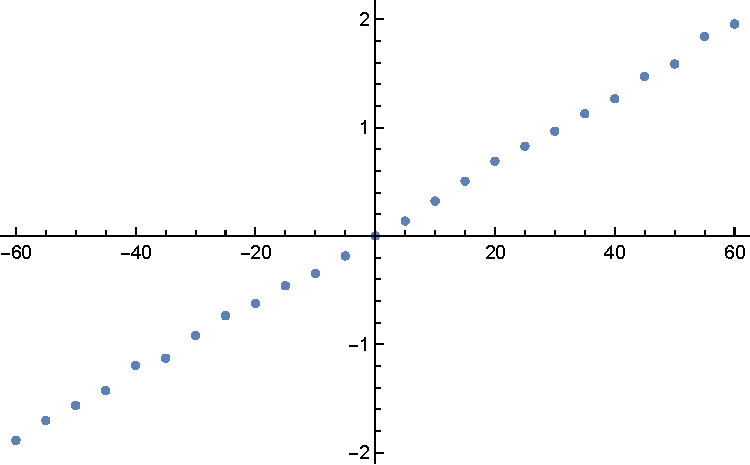
\includegraphics[width=\textwidth]{../Mathematica/images/Pendulo-Pontos.pdf}
\caption{Gráfico exibindo as medidas realizadas}
\label{fig:pendulo-medidas}
\end{figure}

É fácil observar que há uma tendência linear nas medidas, então podemos realizar um ajuste de curvas a fim de tentar obter a reta que melhor representa os dados medidos. Na equação \ref{eq:pendulo-model} temos o modelo de curva que fornece o melhor ajuste:

\begin{equation}
	V(\theta) = 0.0318532 \theta +0.02116
	\label{eq:pendulo-model}
\end{equation}

onde $V(\theta)$ é a tensão elétrica do pêndulo e $\theta$ é o angulo do pêndulo em graus.

Com esta equação também é possível calcular a sua função inversa e obter o ângulo em função da tensão elétrica, na equação \ref{eq:pendulo-model-inverse}, a função inversa do modelo é dada:

\begin{equation}
	\theta(V) = -0.664297 + 31.394 V
	\label{eq:pendulo-model-inverse}
\end{equation}

Dessa forma, podemos utilizar a equação \ref{eq:pendulo-model-inverse} para calcular o angulo de um pêndulo em função de seu correspondente valor de tensão elétrica conforme será feito a seguir.

A fim de obter uma curva de tensão elétrica em função do tempo, desenvolvemos uma aplicação no LABView que fosse capaz de exibir a curva extraída em tempo real na tela e pudesse exportar estes dados de forma que pudessem ser processados externamente. Na figura \ref{fig:pendulo-labview} está mostrado uma imagem do programa utilizado.

\todo{adicionar um print do labview}

Após realizar a exportação dos dados utilizamos o software Wolfram Mathematica para importar estes dados em formato TSV (tab-separated values) e realizar o processamento. Primeiramente, precisamos notar que a informação importada está em valores de tensão elétrica (Volt) e tempo (segundo). Primeiramente, desejamos converter estes valores de tensão elétrica em uma posição angular do pêndulo e para isto, utilizamos a função inversa calculada na equação \ref{eq:pendulo-model-inverse} e a aplicamos a cada ponto medido pelo DAQ pelo LABView.



\chapter{Conclusões}

\chapter*{Anexos}
\section{Mathematica}
\includenotebook{../Mathematica/Experimento 1-1.pdf}{Experimento 1}

\section{LabVIEW}

\section{MATLAB}

\begin{thebibliography}{9}
\bibitem{mathematica-numerial-precision} \url{https://reference.wolfram.com/language/tutorial/NumericalPrecision.html}, acessado em 16 de março de 2016
\bibitem{ref1} Sobrenome, A.B.; Sobrenome, C.D. Title of the cited article. Journal Title 2007, 6, 100-110. 
\bibitem{ref2} Balbinot, A.; Brusamarello, V.J.. Title of the cited article. Journal Title 2007, 6, 100-110. 
\bibitem{ref3} Author, A.; Author, B. Title of the chapter. In Book Title, 2nd ed.; Editor, A., Editor, B., Eds.; Publisher: Publisher Location, Country, 2007; Volume 3, pp. 154-196.
\bibitem{ref4} Author, A.; Author, B. Book Title, 3rd ed.; Publisher: Publisher Location, Country, 2008; 
pp. 154-196.
\todo{arrumar bibliografia}

\end{thebibliography}

\end{document}
